\documentclass{article}

\usepackage{Paper}
\pdftitle{Waste-PhiPhi}

% === TITLE ===
\title{\textbf{Waste Management in the Phi Phi Islands, Thailand \\ Waste Management and Recycling}}
\author{Matteo Frongillo, Antonio Monti, Michael Moos}
\date{}

% === TEXT ===
\begin{document}
\hypersetup{citecolor=black}
\maketitle

\section*{Context}
\begin{itemize}
    \item \textbf{Tourism pressure:} Mass tourism, popularised by ``The Beach'', and seasonal visitor peaks place heavy pressure on the islands' waste services.
    \item \textbf{Limited infrastructure:} Inadequate collection, minimal recycling, and limited disposal and treatment capacity lead to open burning, uncontrolled dumping, and marine pollution.
    \item \textbf{Main drivers:} Over-tourism, day trips from Phuket and Krabi, limited space, and widespread use of single-use plastics in food and beverage outlets.
    \item \textbf{Key stakeholders:} Tourists, residents, local government, hotels, tour operators, and restaurants.
    \item \textbf{Risks if unresolved:} Loss of tourist appeal and income; damage to coral reefs and plastic ingestion by marine species; air pollution from burning and contamination of water supplies.
\end{itemize}

\section*{Question 1}
\begin{center}[H]
    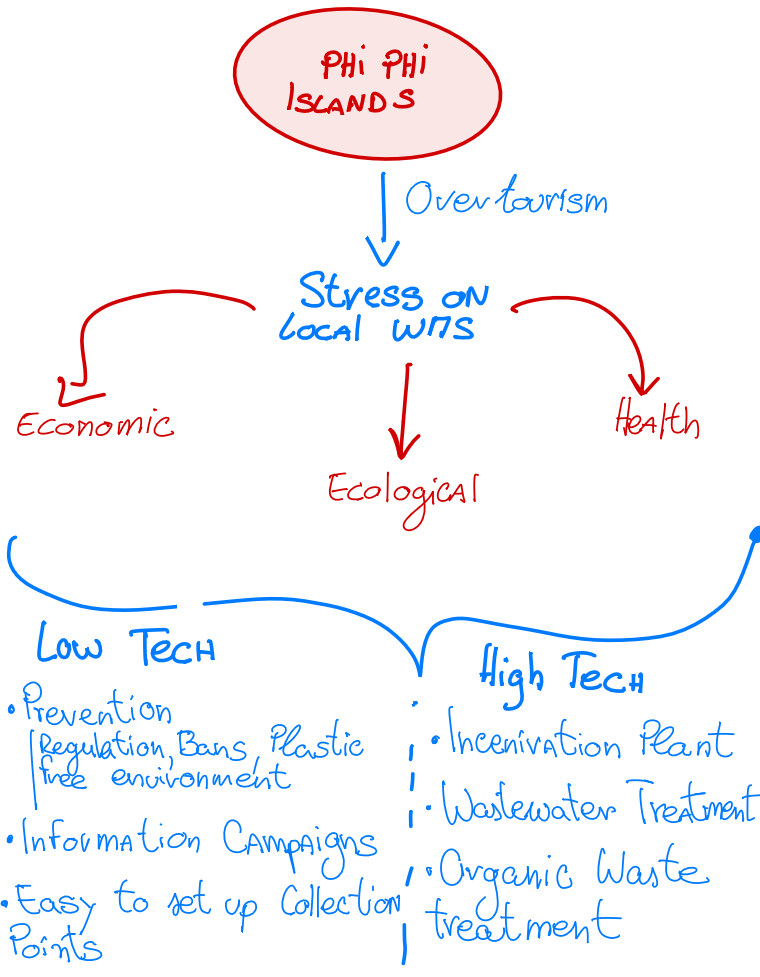
\includegraphics[\lw]{phiphi.png}
\end{center}

\newpage
\section*{Question 2}
\begin{center}
    Reduce $\to$ separate $\to$ collect properly $\to$ recycle/threat $\to$ dispose safely
\end{center}
This would be a feasible alternative to more high tech solutions
such as wastewater treatment plants and incineration plants.
With relatively simple measures the Government can improve the
actual situation while also adressing the shortage of resources
wetehr that be technology or financial.

\section*{Question 3}
The government is the main responsible, as it should provide
infrastructures and rules to mitigate the over-tourism problem.

Tourism businesses should pay the social costs.

Tourists and residents should follow the local rules.

\end{document}
